\section{The problem}
We have to solve to following problem:
 
\medskip 
\scriptsize
\framebox[15cm]{ %
\begin{minipage}{140mm}
Build a distributed system composed of a Button and a Led, each controlled by a different computational node.
The system must initially provide a very basic function: a Led is turned on and off each time a Button is pressed (by an human user). 

In the future, the functionalities of the systems could be extended, e.g. by allowing a Button to blink a Led, to turn on/off many Led etc.
\end{minipage}}
\normalsize
\medskip    

We read the text file that describes the requirements and immediately plan some work to:

\begin{itemize}
\item define the model of the Led (question: \textit{what} is a Led in the user domain space?);
\item define the model of the Button (question: \textit{what} is a Button in the user domain space?);
\item define the (model of the) Use Cases (i.e. define the functions/features of the software system).
\end{itemize}

\subsection{The UseCases.}
The main functions of the software systems can be summarized as done in
\href{https://137.204.107.21/syskb/it.unibo.iss2015intro/docs/Appls/ButtonLed/buttonLedHighLevelEntry.html}{|>>site/BLS usecases}.

\subsection{From Requirement Analysis to the software development process}

After the analysis related to the system components, we ask ourselves whether the models of the Led and of the Button defined in cooperation with the user can be also suited to face the problem of building the required distributed software system. Since it is not the case, we immediately advert a conceptual distance between the basic components and the needs of the application (i.e. we find an \textit{abstraction gap}) that can be reduced by describing the single components and the whole system by means of a custom meta-model, no more based on classical objects but on \textit{actors}.

In the following, we will show how a proper requirement analysis staring from the system components, properly related to the problem analysis and formally expressed by (executable) models can provide a solid guide for agile (\texttt{SCRUM}-based) project and implementation phases by reducing the risks and the costs for the software company.

\newpage 
\section{The Led (as basic logical device)}
\labelsec{led}
In the application domain of the customer, the Led is a physical device (see
\href{https://137.204.107.21/syskb/it.unibo.iss2015intro/docs/Appls/ButtonLed/LedEntry.html}{|>>site/LedEntry}) that can be modelled  as a \textit{Plain Old Java Object} (see \href{https://en.wikipedia.org/wiki/Plain_Old_Java_Object}{net/POJO} ).


\subsection{The Led as a \texttt{POJO}}
%
More precisely, we can state that a Led is an object with a modifiable state that can provide (implement) the following interface:

%%\begin{Verbatim}[fontsize=\scriptsize, frame=single]
\begin{lstlisting}
public interface ILed {
  public String getName();             // property , primitive	
  public void turnOn();                // modifier , primitive
  public void turnOff();               // modifier , primitive
  public java.awt.Color getLedColor(); // property , primitive
  public boolean isOn();               // property , primitive
  public void doSwitch();              // non-primitive
  public String getDefaultRep();       // mapping , non-primitive
}
\end{lstlisting}
%%\end{Verbatim}

The comments near each operation give some first indication on the intended semantics of the operation according with the terminology reported in \href{https://137.204.107.21/syskb/it.unibo.iss2015intro/docs/NatMolBook/content/book/sistemi/comportamentoSistemi.html}{book/ops	})

%% \lstinputlisting[language=java,caption={ \texttt{ILed.java} }, firstline=1 ]{../../../it.unibo.buttonLedSystemHL/src/it/unibo/bls/lowLevel/interfaces/ILed.java}

%% \lstinputlisting[language=java,caption={ \texttt{IDeviceLedImpl.java} }, firstline=1 ]{../../../it.unibo.buttonLedSystemHL/src/it/unibo/bls/lowLevel/interfaces/IDeviceLedImpl.java}

%% At the very first stage of development, the \texttt{ILed} interface and the  is introduced without any need to define a \texttt{IDeviceLedImpl}. However, since our software company is working in the \texttt{IOT} (\textit{Internet of Things}) filed, it has already defined a reusable taxonomy for \texttt{IOT} devices, according to the model discussed in \xss{devbridge}.

\subsection{The Led model test-plan}
\labelssec{ledtestplan}
However, the usage of comments is not the best way to specify the intended semantics of an operations.
By recalling the motto of Young et al. (1985):

\medskip 
\scriptsize
\framebox[15cm]{ %
\begin{minipage}{140mm}
A design without specifications cannot be right or wrong, it can only be surprising! 
\end{minipage}}
\normalsize
\medskip 


our next step is to immediately introduce a test plan (see  \href{https://137.204.107.21/syskb/it.unibo.iss2015intro/docs/NatMolBook/content/book/modelBased/fasi/pianoCollaudo.html}{book/test plans}), to better specify the expected  behaviour (i.e. the meaning) of each operation.

The test plan that follows is directly expressed in \texttt{JUnit} (see 
\href{http://www.vogella.com/tutorials/JUnit/article.html}{net/JUnit tutorial}) even if we do not have, at this moment, nothing to test. The idea is to use each test as a \textit{specification} of the expected behaviour and as a way to express in a more formal way what each operation should do.

\lstinputlisting[language=java,caption={ \texttt{A Test Plan for the Led} }, firstline=1 ]{../../../it.unibo.buttonLedSytem.tests/src/it/unibo/buttonLedSytem/tests/TestLed.java}

%%\href{https://137.204.107.21/syskb/it.unibo.iss2015intro/docs/NatMolBook/Testing.html}{testing}), to better specify the expected behaviour of each Led operation:

\subsection{The Led as an actor (problem analysis)}
\labelssec{ledasactor}
The current model of the Led as a \texttt{POJO} does not include any capability to interact via the network  with the other components of the system. In other words, this model is not able to capture the distributed nature of the system.

In the context of a distributed button-led system, the Led could be conceived as a more advanced device, modelled as an \textit{actor} able to receive and execute command messages. 
%
This new model can be expressed by using the \texttt{qa} metamodel as follows:
\lstinputlisting[language=ddr,caption={ \texttt{ledMsg.qa} }, firstline=1 , lastline=31]{../../../it.unibo.bls2016.led/src/ledMsg.qa}

The \texttt{ledmsg} actor is a state machine that first performs a configuration phase and then works in a message-based way.
% 
In the configuration phase the actor load a theory (\texttt{ledTheory}) and creates a (\texttt{POJO}) Led, that will be updated by calling \tuprolog{} rules (\texttt{turnTheLed/1} or \texttt{turnOn/turnOff}) defined in the \texttt{ledTheory}.

Thus, the idea of a Led as a \texttt{POJO} is not abandoned; it is simply included (embedded) into the more advanced concept of \texttt{ledmsg} actor.

\subsection{The Led (configuration) \texttt{ledTheory} }
\labelssec{ledTheory}
The main task of the \texttt{ledTheory} is done during its \textit{initialization}: load a specific led-theory for each Led implementation:

\lstinputlisting[language=ddr,caption={ \texttt{ledTheory.pl} }, firstline=1 ]{../../../it.unibo.bls2016.led/ledTheory.pl}

If no \texttt{ledImplementation/1} fact is defined within the \texttt{ledTheory}, then we do not have any concrete Led implementation to use, as usually happens during the requirement or problem analysis phase. Nevertheless, we aim at introducing a working model even in this early phase of software development, in order to better interact with the user and to fix the requirements as soon as possible. For this reason the \texttt{ledTheory} loads a \texttt{ledNoImplTheory}. 

\subsection{A first Led (implementation) object}

The \texttt{ledNoImplTheory}  models the led state as a fact \texttt{ledState/1} and 'implements' the Led operations by introducing a proper set of rules:

 
%% The \texttt{ledTheory} is introduced to link the abstract view of the Led as an actor to some 'concrete' device (object), implemented with some specific technology; for example, we could introduce a physical Led controlled by an Arduino or a Raspberry or a virtual Led implemented by a GUI, and so on. 

%% However, when we are in the requirement or problem analysis phase, we should avoid to enter in any technological detail at this stage; nevertheless, we aim at introducing a working model even in this early phase of software development, in order to better interact with the user and to fix the requirements as soon as possible.

%% For this reason we model the led state as a fact \texttt{ledState/1} and 'implement' the Led by introducing a proper set of rules. 

\lstinputlisting[language=ddr,caption={ \texttt{ledNoImplTheory.pl} }, firstline=1 ]{../../../it.unibo.bls2016.led/ledNoImplTheory.pl}

This theory defines a very simple implementation of the Led as a \texttt{POJO}, by introducing rules related to the \texttt{ILed} interface of \xss{ledtestplan}. 


In this way, we are able to build a working prototype of a basic component (and later of the whole system) in a short time still during requirement analysis; even the unit test plans of \xss{ledtestplan} can be included in the component prototype.

The \texttt{createLed/2} rule is by now defined by asserting some facts in the knowledge base. This rule will be proprerly re-defined in each specific Led implementation theory, in order to introduce a specific concrete device, for example the \texttt{LedMock} used in the test plan of \xss{ledtestplan}.
 
%%Since we can have several Led implementation, we associate a theory to each type of Led implementation and use a rule to detect and load the proper theory:

%%\lstinputlisting[language=ddr,caption={ \texttt{ledTheory.pl} }, firstline=1 ]{../../../it.unibo.bls2016.led/ledTheory.pl}

\subsection{Testing the actor Led component} 
The Led component model can be executed by adding in the \texttt{qa} model a simple message generator (that will be later replaced by a button or by some other input  device):
\lstinputlisting[language=ddr,caption={ \texttt{ledMsg.qa extended with a Led command generator } }, firstline=32 ]{../../../it.unibo.bls2016.led/src/ledMsg.qa}

\subsection{A Mock Led (project/implementation phase)}
\labelssec{ledmock}

Our software company has already developed an implementation for a mock object\footnote{In object-oriented programming, \textit{mock objects} are simulated objects that mimic the behaviour of real objects in controlled ways.}  for the Led :

\lstinputlisting[language=java,caption={ \texttt{LedMock.java} }, firstline=1 ]{../../../it.unibo.buttonLedSystemHL/src/it/unibo/buttonLed/components/LedMock.java}

Since this class is the result of some project or implementation phase, a lot of work has been already done to enhance code reusability. In particular, the software team has introduced the class \texttt{DeviceLedImpl} (see  \xss{DeviceLedImpl} ) as a basic class for all the different types of Led implementations; in this way, for each specific Led implementation we have to redefine some operation only (in this case the internal operation \texttt{show}). 

In order to 'inject' this new implementation of the Led into our logical component, we define the theory \texttt{ledMockTheory} with a specific \texttt{createLed/2} rule: 


\lstinputlisting[language=ddr,caption={ \texttt{ledMockTheory.pl} }, firstline=1 ]{../../../it.unibo.bls2016.led/ledMockTheory.pl}

The next step is to introduce two new rules in  the \texttt{ledTheory} of \xss{ledTheory}:

%%\begin{Verbatim}[fontsize=\scriptsize, frame=single , label=Facts related to \texttt{LedMock} in \texttt{ledTheory	}]
\begin{lstlisting}
ledImplementation( mock ).
...
ledImplementationFile( mock, "ledMockTheory.pl"   ).
\end{lstlisting}
%%\end{Verbatim}

\newpage 
\section{A Led factory }
\labelssec{DeviceLedFactoryQa}
The \java{} class \texttt{DeviceLedFactoryQa} used in the \texttt{LedMock} of \xss{ledmock} is a \textit{factory} that provides static methods to create a \textit{singleton} Led object and to get a reference to such an object:

\lstinputlisting[language=java,caption={ \texttt{DeviceLedFactoryQa.java : createLedMock} }, firstline=1 , lastline=25]{../../../it.unibo.bls2016.device.qa/src/it/unibo/devices/qa/DeviceLedFactoryQa.java}

Note that the creation method \texttt{createLedMock} returns (like any other creation method that we will introduce in the factory) an object of the class \texttt{DeviceLedImpl} (see  \xss{DeviceLedImpl} ). 

\subsection{The Led usage theory }
Since we have introduced a factory that builds and gets objects of class  \texttt{DeviceLedImpl}, we can write a set of Led-usage rules that do not depend on the specific Led implementation:

\lstinputlisting[language=ddr,caption={ \texttt{ledUsageTheory.pl} }, firstline=1 ]{../../../it.unibo.bls2016.led/ledUsageTheory.pl}

\subsection{A basic class for Led implementation}
\labelssec{DeviceLedImpl}
The \texttt{DeviceLedImpl} class is based on the custom framework \href{https://137.204.107.21/syskb/it.unibo.iss2015intro/docs/Frameworks/FramwCustomAppl.html}{|>>site/uniboEnv}) introduced for the rapid development of \texttt{GUI}-based prototypes.

\lstinputlisting[language=java,caption={ \texttt{DeviceLedImpl.java} }, firstline=1 ]{../../../it.unibo.buttonLedSystemHL/src/it/unibo/buttonLed/components/DeviceLedImpl.java}


\subsection{A Virtual Led (project/implementation phase)}

A Led as a virtual device can now be introduced as follows:

%%\lstinputlisting[language=java,caption={ \texttt{DeviceLedGui.java} }, firstline=1 ]{../../../it.unibo.buttonLedSystem.gui/src/it/unibo/buttonLedSystem/gui/DeviceLedGui.java}

The class  \texttt{DeviceLedImpl} redefines two internal operations: \texttt{configure} and \texttt{show}. The result is shown in the following picture:

%%This implementation is a specialized version of the more general Led implementation class (\texttt{DeviceLedImpl},see  \xss{DeviceLedImpl} ) that changes the size of a picture when the Led changes its state.

\begin{center}
\begin{tabular}{ c }
     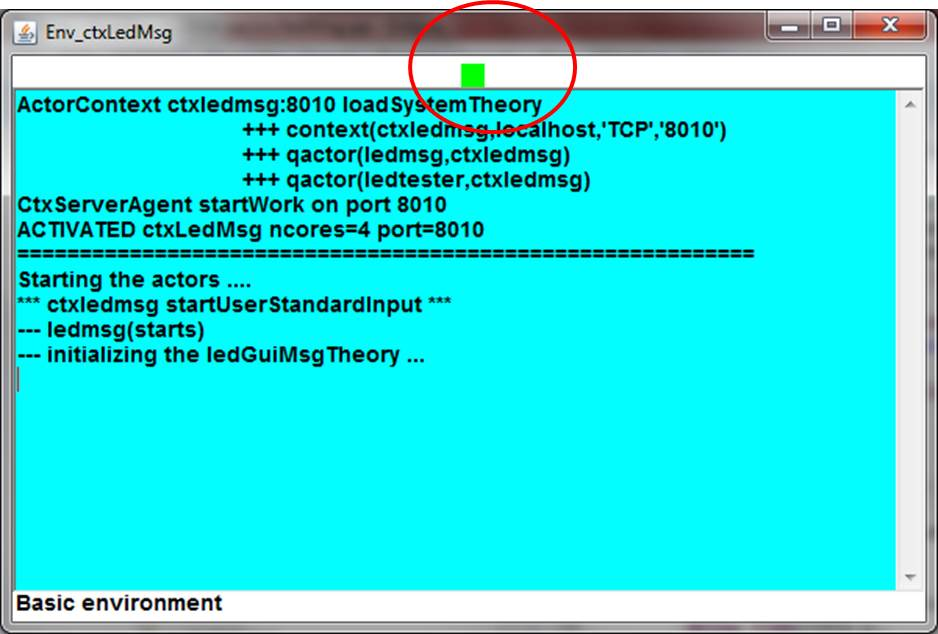
\includegraphics[scale = 0.45]{./img/ledGui.jpg}\\
\end{tabular}{   }
\end{center}

In order to 'inject' this new implementation of the Led into our logical component, we define the theory \texttt{ledGuiTheory} with a specific \texttt{createLed/2} rule: 


\lstinputlisting[language=ddr,caption={ \texttt{ledGuiTheory.pl} }, firstline=1 ]{../../../it.unibo.bls2016.led/ledGuiTheory.pl}

The next step is to introduce two new rules in  the \texttt{ledTheory} of \xss{ledTheory}:

%%\begin{Verbatim}[fontsize=\scriptsize, frame=single , label=Facts related to \texttt{LedGui} in \texttt{ledTheory	}]
\begin{lstlisting}
ledImplementation( gui ).
...
ledImplementationFile( gui,  "ledGuiTheory.pl"   ).
\end{lstlisting}
%%\end{Verbatim}
 
Finally, we introduce a new Led creation operation in the entry in the \texttt{DeviceLedFactoryQa}:
\begin{lstlisting}
    public static DeviceLedImpl createLedGui(  
    		 String name, IOutputEnvView outEnvView, int color) throws Exception{
     	if( myself == null ){
  	  		LedColor ledcolor = (color == 0) ? LedColor.GREEN : LedColor.RED ;
	  		myself = new DeviceLedGui(name,outEnvView, ledcolor);  			 
  		}
  		return myself;
   	}
\end{lstlisting}
\newpage 
\section{A Led on Raspberry (implementation phase)}
The \texttt{GPIO} pins on a Raspberry Pi are a great way to interface physical devices like Buttons and Leds through some simple hardware connection, as in the example described in
%\href{https://137.204.107.21/syskb/it.unibo.iss2015intro/docs/Raspberry/pi4j.html}{|>>site/Pi4j}) and 
\href{https://137.204.107.21/syskb/it.unibo.iss2015intro/docs/Appls/ButtonLed/buttonLedLowLevel.html}{|>>site/BLS low-level})). In this example the Led anode  is connected to pin \texttt{25} in \texttt{BCM} code\footnote{\texttt{BCM} refers to the pin number of the \texttt{BCM2835} chip, and this is the pin number used when addressing the \texttt{GPIO} using the \texttt{/sys/class/gpio} interface}  while the Led cathode is connected to a \texttt{GND} pin.

However, a software design never interacts in direct way with the hardware level; at least some minimal support for the control of external devices must be provided by the operating system. In the case of Linux we can start from the shell or from a more advanced library.


\subsection{Led control using files}
The basic way provided by Linux to manage a device connected on a \texttt{GPIO} pin is reading/writing some (virtual) file associated with that pin.

\lstinputlisting[language=ddr,caption={ \texttt{led25OnOff.sh} }, firstline=1 ]{../../../it.unibo.raspIntro/src/it/unibo/bls/bash/led25OnOff.sh}

\subsection{Led control using the \texttt{GPIO} shell library}
\textit{WiringPi} is a \texttt{GPIO} access library written in \texttt{C}\footnote{The \textit{WiringPi}  library was written by Gordon Henderson to allow \texttt{GPIO} communication from \texttt{C,C++} in a style similar to the Arduino Wiring programming language} for the \texttt{BCM2835} used in the Raspberry Pi. \textit{WiringPi} includes a command-line utility \texttt{gpio} which can be used to program and setup the \texttt{GPIO} pins. We can use this to read and write the pins and even use it to control them from shell scripts.

\lstinputlisting[language=ddr,caption={ \texttt{led25Gpio.sh} }, firstline=1 ]{../../../it.unibo.raspIntro/src/it/unibo/bls/bash/gpio/led25Gpio.sh}

\subsection{Led control using python}
The Raspbian Linux operating system  has the \texttt{RPi.GPIO} library pre-installed. It is a Python library that handles interfacing with the \texttt{GPIO} pins.

\lstinputlisting[language=ddr,caption={ \texttt{ledPython25.sh} }, firstline=1 ]{../../../it.unibo.raspIntro/src/it/unibo/bls/python/ledPython25.py}

 \subsection{Led control using Pi4j}
\texttt{Pi4J} is an open source project  intended to provide a bridge between the native hardware and \java{} for full access to the Raspberry Pi. In addition to the basic raw hardware access functionality, this project also attempts to provide a set of advanced features that make working with the Raspberry Pi an easy to implement and more convenient experience for \java{} developers.

Thus, the \texttt{Pi4J} library (see \href{https://137.204.107.21/syskb/it.unibo.iss2015intro/docs/Raspberry/pi4j.html}{|>>site/Pi4j}) can be used as our basic software layer (our \textit{technology assumption}) for the implementation a \java{} class for the control of a Led connected to some pin of a Raspberry Pi:

\lstinputlisting[language=java,caption={ \texttt{DeviceLedPi4j.java} }, firstline=1 , lastline=50]{../../../it.unibo.buttonLedSystem.raspberry/src/it/unibo/bls/raspberry/components/DeviceLedPi4j.java}

In this case the class redefines two primitive operations of \texttt{DeviceLedImpl} (see \xss{DeviceLedImpl}): \texttt{turnOn} and \texttt{turnOff}. Moreover, it extends the configuration phase by 'provisioning' (in \texttt{Pi4j} terminology) the \texttt{GPIO} pin connected to the Led anode. 
%
The class \texttt{GpioOnPi4j} is an utility class that maps a \texttt{GPIO} pin number in \texttt{BCM}  into a \textit{wiring Pi} code:

\lstinputlisting[language=java,caption={ \texttt{GpioOnPi4j.java} }, firstline=1 , lastline=54]{../../../it.unibo.bls2016.device.qa/src/it/unibo/gpio/base/GpioOnPi4j.java}

\subsection{Using the Led Pi4j in the actor}
In order to 'inject' this new implementation of the Led into our logical component, we define the theory \texttt{ledPi4jTheory.pl}:

\lstinputlisting[language=ddr,caption={ \texttt{ledPi4jTheory.pl} }, firstline=1 ]{../../../it.unibo.bls2016.led/ledPi4jTheory.pl}

The next step is to introduce two new rules in  the \texttt{ledTheory} of \xss{ledTheory}:

%%\begin{Verbatim}[fontsize=\scriptsize, frame=single , label=Facts related to \texttt{LedMock} in \texttt{ledTheory	}]
\begin{lstlisting}
ledImplementation( rasp ).
...
ledImplementationFile( rasp, "ledPi4jTheory.pl"  ).
\end{lstlisting}
%%\end{Verbatim}

Finally, we introduce a new Led creation operation in the entry in the \texttt{DeviceLedFactoryQa}:
\begin{lstlisting}
    public static DeviceLedImpl createLedPi4j( 
    		 String name, IOutputEnvView outEnvView, int color, int pinNum) throws Exception{
      	if( myself == null ){
    		LedColor ledcolor = (color == 0) ? LedColor.GREEN : LedColor.RED ;
  	  		myself = new DeviceLedPi4j( name,outEnvView, ledcolor, pinNum);  			 
   		}
   	    return myself;
    }
\end{lstlisting}

\subsection{Code deployment on the Raspberry Pi}
In order to test our code on the Raspberry Pi we have to perform the following actions:
\begin{enumerate}
\item create a runnable \texttt{jar} file from the generated file \texttt{src-gen/it/unibo/ctxLedMsg/MainCtxLedMsg.java}\footnote{We suggest to copy the required libraries in a sub-folder to keep the \texttt{jar} short and to reduce the time of file transfer to the Raspberry Pi.};
\item copy the runnable \texttt{jar} and the library sub-folder into a directory (e.g. \texttt{ledTest}) the Raspberry Pi;
\item copy the generated \texttt{scrMore} directory into \texttt{ledTest};
\item copy the into \texttt{ledTest} the theories  \texttt{ledTheory.pl}, \texttt{ledMockTheory.pl}, \texttt{ledGuiTheory.pl} \texttt{ledPi4jTheory.pl} and \texttt{ledUsageTheory.pl}.
\end{enumerate}

\subsection{Test the Led on the Raspberry Pi}
The behaviour of the Led component on the Raspberry Pi can be tested by launching (within the directory \texttt{ledTest}):

\begin{Verbatim}[fontsize=\scriptsize, frame=single , label=Launch the Led test]
sudo java -jar MainCtxLedMsg
\end{Verbatim}

We can select one of the different Led implementations by setting one of the \texttt{ledPi4jTheory.pl} implementation rules:

\begin{Verbatim}[fontsize=\scriptsize, frame=single , label=Select the Led implementation]
%% ledImplementation( mock ).
%% ledImplementation( gui ).
ledImplementation( rasp ).
\end{Verbatim}

The system with the rule \texttt{ledImplementation( gui )} works only under a \texttt{X11} system\footnote{The\textit{ X Window System} (\texttt{X11}, or shortened to simply \texttt{X}, and sometimes informally \texttt{X-Windows}) is a windowing system for bitmap displays, common on \texttt{UNIX}-like computer operating systems} to enable remote graphical access to applications.

\subsection{The Led as a standalone device}
Since we now have a Led working on a Raspberry Pi, we can immediately switch from a local system to a distributed one. To this end, let us introduce an actor that, working on a conventional \texttt{PC}, sends command messages to the Led on the Raspberry Pi:

\lstinputlisting[language=ddr,caption={ \texttt{ledSenderMsg.qa} }, firstline=1 , lastline=31]{../../../it.unibo.bls2016.led/src/ledSenderMsg.qa}

Note that the \texttt{ledtester} is identical to the actor introduced in  \xss{ledasactor}, with the difference that it works in its own Context \texttt{ctxLedSenderMsg}. Moreover, the behaviour of the \texttt{ledmsg} actor is \textbf{not} explicitly defined; rather a 'place holder' actor is introduced in the specification in order to:
\begin{enumerate}
\item allow us to reference the \texttt{ledmsg} actor in a message send (\texttt{forward}) operation;
\item define the context (in practice, the \texttt{IP} of the Raspberry Pi) in which the \texttt{ledmsg} is working.
\end{enumerate}

The flag \texttt{-standalone}  indicates that the Led context \texttt{ctxLedMsg} must be considered an entity outside the system and that the actors defined in it are just 'place holders' that do not produce any new code. More on this in \xs{dynsys}.

 
\newpage 
\section{A Led on Arduino (implementation phase)}
The basic way provided by Arduino to manage a device connected on a pin is to perform a read or a write operation on that pin. For example we can blink a Led connected on pin \texttt{13} as follows:

\lstinputlisting[language=java,caption={ \texttt{Led13.ino}}, firstline=1  ]{../../../it.unibo.arduino.intro/Arduino/programs/Led13/Led13.ino} 

\subsection{Led with input output} 

The next \textit{sketch} does introduce a \texttt{cmdHandler} operation that looks at the serial line as an input device and turns the Led \texttt{on/off} if the input value is \texttt{1/0}.

\lstinputlisting[language=java,caption={ \texttt{Led13Msg.ino}}, firstline=1  ]{../../../it.unibo.arduino.intro/Arduino/programs/Led13Msg/Led13Msg.ino} 



\subsection{DeviceLedArduinoProxy} 
The possibility to send/receive information via the Serial Line can be used as our basic software layer (our \textit{technology assumption}) for the implementation a \java{} class for the control of a Led connected to some pin of a Arduino device. To achieve the goal let us introduce a new specialized version of the \texttt{DeviceLedImpl} (see \xss{DeviceLedImpl}) class:


\lstinputlisting[language=Java,caption={ \texttt{DeviceLedArduinoProxy.java} }, firstline=1 ]{../../../it.unibo.bls2016.device.qa/src/it/unibo/devices/qa/DeviceLedArduinoProxy.java}

The class \texttt{DeviceLedArduinoProxy}\footnote{In computer programming, the \textit{proxy} pattern is a design pattern. A proxy, in its most general form, is a class functioning as an interface to something else.} redefines two primitive operations: \texttt{turnOn} and \texttt{turnOff}. 
%
Moreover, it extends the configuration phase by creating an object of interface \texttt{IConnInteraction} in order to use the serial connection with Arduino.\footnote{The \textit{Java Simple Serial Connector} (\texttt{jscc}) library  is required. It is an evolution of \texttt{RxTx}, see \href{https://blogs.oracle.com/jtc/entry/java_serial_communications_revisited}{net/jSSC}.} 

\subsection{IConnInteraction interface} 
The interface \texttt{it.unibo.is.interfaces.protocols.IConnInteraction} defines operations to send/receive Strings over a  network connection.

\lstinputlisting[language=java,caption={ \texttt{IConnInteraction.java} }, firstline=1 ]{../../../it.unibo.interfaces/src/it/unibo/is/interfaces/protocols/IConnInteraction.java}

The project \textit{it.unibo.noawtsupports} defines a framework for network communications based on connected, two-way protocols (like \texttt{TCP}, \texttt{UDP}) and over a serial line.

The factory \texttt{it.unibo.supports.FactoryProtocol} creates objects of type \texttt{IConnInteraction} that hide the technological details related to specific protocols.  More information on this framework can be found in \href{https://137.204.107.21/syskb/it.unibo.iss2015intro/docs/Readings/UniboSupports/UniboSupports.pdf}{book/UniboSupports.pdf}.

\subsection{Using the serial line in the actor}
In order to 'inject' this new implementation of the Led into our logical component, we define the theory \texttt{ledSerialTheory.pl}:

\lstinputlisting[language=java,caption={ \texttt{ledSerialTheory.pl} }, firstline=1 ]{../../../it.unibo.bls2016.led/ledSerialTheory.pl}

The next step is to introduce two new rules in  the \texttt{ledTheory} of \xss{ledTheory}:

%%\begin{Verbatim}[fontsize=\scriptsize, frame=single , label=Facts related to \texttt{LedMock} in \texttt{ledTheory	}]
\begin{lstlisting}
ledImplementation( serial ).
...
ledImplementationFile( serial, "ledSerialTheory.pl"  ).
\end{lstlisting}
%%\end{Verbatim}

Finally, we introduce a new Led creation operation in the entry in the \texttt{DeviceLedFactoryQa}:
\begin{lstlisting}
    public static DeviceLedImpl createLedSerialProxy( 
   		 String name, IOutputEnvView outEnvView, int color, String portName) throws Exception{
       	if( myself == null ){
       		LedColor ledcolor = (color == 0) ? LedColor.GREEN : LedColor.RED ;
 	  		myself = new DeviceLedArduinoProxy( name, ledcolor, portName, outEnvView);  				 
  		}
       	return myself;
   }
\end{lstlisting}

\newpage 
\section{The Led controlled via a Web page}
\labelsec{ledWeb}
In the \texttt{qa} model of the Led, the flag \texttt{-httpserver} can be introduced in a Context declaration to specify that it must provide a built-in support for web-based interaction. 

\lstset{language=ddr}
\begin{lstlisting}
/*
 * ledMsg.qa
 * This is A MODEL defined during REQUIREMENT or PROBLEM ANALYSIS 
 * by using the qa CUSTOM meta-model / language
 */       
System ledMsg -regeneratesrc      
Dispatch turnLed   : turnLed(X)

Context ctxLedMsg ip [host="localhost" port=8010] -g cyan   -httpserver
...
\end{lstlisting}
\lstset{language=java}

%% \subsubsection{The generated HttpServer.}
When the \texttt{-httpserver} flag is set, a simple \texttt{HTTPserver}\footnote{The class of the server is \texttt{it.unibo.qactors.web.QActorHttpServer})}  is created and started during the Context configuration phase. This server  is based on the \texttt{WebSocket} technology \footnote{The \textit{WebSocket} specification defines an \texttt{API} establishing "socket" connections between a web browser and a server, i.e. a persistent client-server connection so that  both parties can start sending data at any time.} and answers to \texttt{HTTP} requests on port \texttt{8080} by returning the web page named \texttt{QActorWebUI.html} stored in the context package generated in the \texttt{srcMore} directory. 

\subsection{The default page} 
The built-in page has the following aspect:

\begin{center}
\begin{tabular}{ c }
     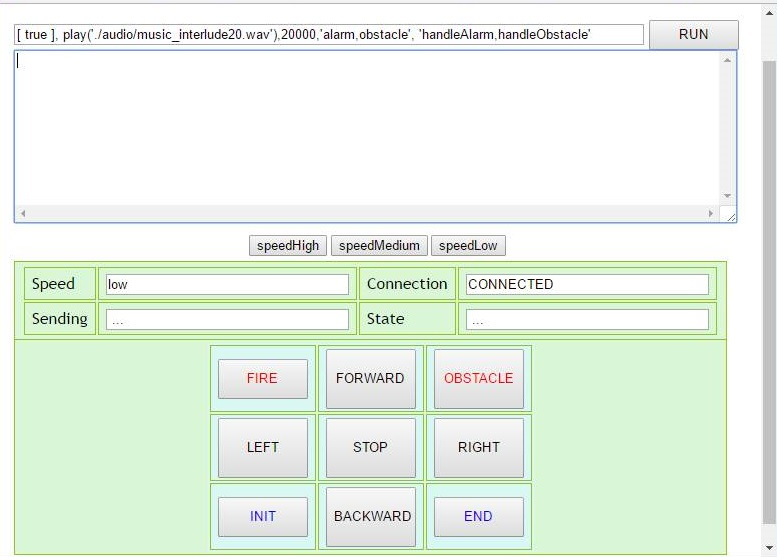
\includegraphics[scale = 0.60]{img/guiweb.jpg}\\
\end{tabular}{   }
\end{center}

The application designer can define (and modify) the content of the \texttt{QActorWebUI.html}  page in order to interact with a QActor by exploiting a conventional Web Browser.

\subsection{A \texttt{HTML} page for the Led}
Let us define a simple page for Led control:

\lstinputlisting[language=ddr,caption={ \texttt{QActorWebUI.html} for the Led }, firstline=1 ]{../../../it.unibo.bls2016.led/descr/QActorWebUI.html}

The page shows itself as follows:
 
\begin{center}
\begin{tabular}{ c }
     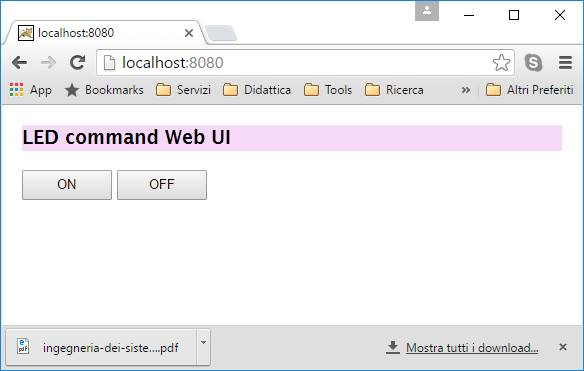
\includegraphics[scale = 0.45]{./img/ledWebGui.jpg}\\
\end{tabular}{   }
\end{center}

The new page for the Led defines two buttons that, once clicked, invoke the \textit{send} operation defined in the \texttt{JavaScript} file \texttt{QActorWebUI.js}:
\lstinputlisting[language=ddr,caption={ \texttt{QActorWebUI.js} for the Led }, firstline=1 ]{../../../it.unibo.bls2016.led/descr/QActorWebUI.js}


\subsection{The work of the built-in QActorHttpServer.} 
 
The \texttt{QActorHttpServer} server handles the input string as follows: 

\lstinputlisting[language=java,caption={ \texttt{QActorHttpServer.java} for the Led }, firstline=156, lastline=165 ]{../../../it.unibo.qactor/src/it/unibo/qactors/web/QActorHttpServer.java} 

Thus, the server performs different actions according to the input string prefix.

\subsection{Input string prefix \texttt{\textbf{m-}}} 
In this case the rest of the input string is assumed to be a \texttt{qa} message of the form:
\medskip
%%\begin{Verbatim}[fontsize=\scriptsize, frame=single , label=]
\begin{lstlisting}
msg( MSGID, MSGTYPE, SENDER, RECEIVER, CONTENT, SEQNUM )
\end{lstlisting}
%%\end{Verbatim}
The \texttt{QActorHttpServer} sends the message to the \texttt{RECEIVER} actor.

For the default page, there no case of this type, that is instead present in the Led web page.

\subsection{Input string prefix \texttt{\textbf{i-}}} 
In this case the rest of the input string is assumed to be a user command (\texttt{CMD}) that is translated into a string of the form:
\medskip   
\begin{Verbatim}[fontsize=\scriptsize, frame=single , label=]
usercmd( executeInput( MOVE ) )
\end{Verbatim}
where \texttt{MOVE} can take one of the following forms:
\medskip
\begin{Verbatim}[fontsize=\scriptsize, frame=single , label=]                                  
[ GUARD ] , ACTION
[ GUARD ] , ACTION , DURATION
[ GUARD ] , ACTION , DURATION , ENDEVENT
[ GUARD ] , ACTION , DURATION , [EVENTLIST], [PLANLIST]
\end{Verbatim}
For the default page, this is the case of the user-command interface; the  \texttt{QActorHttpServer}  emits the following event:

\indent{     } \texttt{usercmd : usercmd(executeInput( CMD ))}	(\texttt{RUN} button) \\

\subsection{Input string without special prefix} 
In this case, the string is assumed to be written in \prolog{} syntax. For the default page, this is the case of the robot-console buttons, that generate input strings of the form:

\begin{Verbatim}[fontsize=\scriptsize, frame=single , label=]
e(alarm(fire))
e(alarm(obstacle))
w( high )
...
\end{Verbatim}
The  \texttt{QActorHttpServer}  emits the following events:  

%% \indent{     } \texttt{inputcmd : usercmd(executeInput( CMD ))} (\texttt{INPUT} button) \\
\indent{     } \texttt{usercmd : usercmd(robotgui(MOVE))} with \texttt{MOVE=w(low),...,s(high)} (\texttt{MOVE} button) \\
\indent{     } \texttt{alarm   : alarm(fire)}  		(\texttt{FIRE} button) \\
\indent{     } \texttt{alarm   : alarm(obstacle)}		(\texttt{OBSTACLE} button)  
 
 
\newpage 
\section{The Button}
\labelsec{button}

As regards the Button, we will follow a  workflow similar to that introduced for the Led in \xs{led} :

\begin{enumerate}
\item model the basic idea of a Button as a \texttt{POJO} component;
\item model the idea of Button required by the problem as an actor;
\item introduce a set of different implementations for the basic button and use them in the proper concrete situation.
\end{enumerate}

\subsection{The Button as a \texttt{POJO}}
\labelssec{ButtonPojo}

In the application domain of the customer, the Button is a physical input device that can be modelled in several ways (a first discussion can be read in \href{https://137.204.107.21/syskb/it.unibo.iss2015intro/docs/Appls/ButtonLed/button.pdf}{|>>site/button.pdf}). 

In this section we start form the idea that a Button is an \textit{observable} (in sense of \texttt{GOF} patterns) \texttt{POJO}.\footnote{See \href{https://137.204.107.21/syskb/it.unibo.iss2015intro/docs/Appls/ButtonLed/buttonEntry.html}{|>>site/buttonEntry}}.
 
%%\subsubsection{The \texttt{IButton} interface.\\}
The Button is then modelled as an entity with some internal modifiable state that can be inspected by all the registered observers or by using the operation \texttt{isPressed}.

%%\begin{Verbatim}[fontsize=\scriptsize, frame=single]
\begin{lstlisting}
public interface IButton {
  public String getName();              // property , primitive	
  public void ispressed();              // property , primitive
  public void addObserver(IObserver o); // modifier
  public String getDefaultRep();        // mapping , non-primitive
}
\end{lstlisting}
%%\end{Verbatim}


%% \subsubsection{The \texttt{IObserver} interface.\\} 

The argument of the operation \texttt{addObserver} must be an 'observer' that implements the following interface:

\lstinputlisting[language=java,caption={ \texttt{IObserver.java} }, firstline=1 ]{../../../it.unibo.interfaces/src/it/unibo/is/interfaces/IObserver.java}

The \texttt{update} operation is called when the state of the button changes.

The interface \texttt{IButton} does not provide any operation to change the internal state of the Button; in fact, the Button should change its state as consequence of some external action. However, it can be wise to introduce some explicit modifier in order to facilitate the testing:

%%\begin{Verbatim}[fontsize=\scriptsize, frame=single]
\begin{lstlisting}
public interface IButton {
	...
	public void high();	//modifier
	public void low();	//modifier
}
\end{lstlisting}
%%\end{Verbatim}

%% An interface for a Button (\texttt{IButton} or \texttt{IDeviceButtonImpl}) 

%% \lstinputlisting[language=java,caption={ \texttt{IButton.java} }, firstline=1 ]{../../../it.unibo.buttonLedSystemHL/src/it/unibo/bls/lowLevel/interfaces/IButton.java}

%% \lstinputlisting[language=java,caption={ \texttt{IDeviceButtonImpl.java} }, firstline=1,lastline=14 ]{../../../it.unibo.buttonLedSystemHL/src/it/unibo/bls/lowLevel/interfaces/IDeviceButtonImpl.java}

%% The interface is defined as a specialization of a more general interface \texttt{IDeviceInputImpl}.

%% \subsubsection{The \texttt{IDeviceInputImpl} interface.\\}
%% The interface \texttt{IDeviceInputImpl} defines the basic operations for any input device intended as an observable entity.

%% \lstinputlisting[language=java,caption={ \texttt{IDeviceInputImpl.java} }, firstline=1 ]{../../../it.unibo.buttonLedSystemHL/src/it/unibo/bls/lowLevel/interfaces/IDeviceInputImpl.java}

%% \subsubsection{The \texttt{IObservable} interface.\\}
 
%% \lstinputlisting[language=java,caption={ \texttt{IObservable.java} }, firstline=1 ]{../../../it.unibo.interfaces/src/it/unibo/is/interfaces/IObservable.java}

%% Besides being observable, the \texttt{IDeviceInputImpl} states that any input device is also an observer and a specialized version of a more general device for \texttt{IOT}\footnote{\textit{Intertnet of Things}}  applications.

%% \subsubsection{The \texttt{IDeviceIot} interface.} 

%% In our input device taxonomy any \texttt{IOT} device must provide (via th operation \texttt{getDefaultRep}) a default representation as a String in some standard syntax like  \texttt{XML}, \texttt{JSON} or \prolog.

%% \lstinputlisting[language=java,caption={ \texttt{IDeviceIot.java} }, firstline=1 ]{../../../it.unibo.interfaces/src/it/unibo/iot/interfaces/IDeviceIot.java}

\subsection{The Button model test-plan}
\labelssec{buttontestplan}

As already done for the Led (see \xss{ledtestplan}), we immediately introduce a test-plan related to the \texttt{IButton} interface as a way to express in a more formal way \textit{what} each operation should do:

\lstinputlisting[language=java,caption={ \texttt{A Test Plan for the Button} }, firstline=1 ]{../../../it.unibo.buttonLedSytem.tests/src/it/unibo/buttonLedSytem/tests/TestButton.java}

\subsubsection{A first observer.\\}

The observer used in the test-plan simply stores the current state of the button:

\lstinputlisting[language=java,caption={ \texttt{ButtonObserverNaive} }, firstline=1 ]{../../../it.unibo.buttonLedSytem.tests/src/it/unibo/buttonLedSytem/tests/ButtonObserverNaive.java}

\subsection{The Button as an actor (problem analysis / project)}
\labelssec{buttonasactor}
The current model of the Button as a \texttt{POJO} does not include any capability to interact via the network  with the other components of the system.  
%
In the context of a distributed ButtonLed system, the Button could be conceived as a more advanced device, modelled as an \textit{actor} able to:
\begin{itemize}
\item emit \textit{events}. In this way any actor can sense or react to state changes of the button ;
\item send \textit{messages} to some other actor, that can be:
\begin{itemize}
\item statically known by the button actor. For example, this is the case of a simple ButtonLed distributed system in which the Button knows the actor Led that must be turned on/off;
\item dynamically acquired by the button actor through some 'registration' message. This is the 'distributed version' of the \texttt{GOF} observer pattern, in which the observable (the Button) does not known a-priori its possible 'remote observers'. 
\end{itemize}
\end{itemize}

As already done for the Led (see \xss{ledasactor}) the Button as a \texttt{POJO} introduced in \xss{ButtonPojo} is not given up; it is still necessary and must be used as a basic support for the behaviour of the Button as an actor. 

\subsection{Fron the Button \texttt{POJO} to the Button actor}
\labelssec{bactorandpojo}

More precisely, the Button-\texttt{POJO} becomes the low-level (technology-dependent)  part of our abstract (technology-independent) concept of Button actor. The 'bridge' between the low-level layer and the logical layer can be delegated to a Button-\texttt{POJO} observer (a \textit{ButtonObserverForActors} - shortly \texttt{BOA} - like that introduced in \xss{bobsqa} ) that can implement a set of different actions:

\begin{enumerate}
\item the \texttt{BOA}  maps a button state change into a \texttt{qa} event. In this case the Button actor works as an active observer of the events emitted by the underlying level;
\item the \texttt{BOA} calls a 'callback' defined in the actor as a Plan. In this case the Button actor logically becomes a passive observer that works as a high-level extension of the underlying \texttt{BOA}\footnote{We could also conceive the Button Actor as an event-driven machine rather than an event-based machine, since a Plan transition occurs without any explicit control.}. The 'callback' Plan does include the 'business logic' related to a change of the button state (e.g. it could send a message to other actors declared in the system model);
\item the \texttt{BOA} immediately performs the 'business logic' by executing some 'script' of the application level. This 'script' could be a rule written in the \textit{WorldTheory} of the Button actor that logically becomes a 'do-nothing' entity.
\end{enumerate}

The last \texttt{BOA} strategy is mentioned here as one as a behaviour 'technically' possible but certainly not advisable, since the behaviour of the Button component cannot be understood at system level. 

This problem does not occur with the second \texttt{BOA} strategy that does minimize computational overheads like the third one. But in this case we must avoid the risk to 'break the model' by mixing the event/message-based nature of the behaviour of an actor with something that looks like as event-driven. This mixing is quite harmful, since we could reintroduce all the problems of concurrent access to shared memory by independent processes that are actually excluded by the event/message-based behaviour of the actors.

The first \texttt{BOA} strategy is the most appropriate at conceptual level, since an actor is an active machine working as a event/message-based finite state machine. However it does introduce computational overhead since the system must generate a \texttt{qa} event and after resume a quiescent actor.

In the following we will show examples of all these kinds of behaviour by introducing rules that assure that, in cases of a \texttt{BOA} strategies \texttt{2} and \texttt{3} the Button actor immediately ends logically 'becoming' a conventional object.

\subsection{The Button as a message sender}

Let us introduce in this section a \texttt{qa} model of the Button that (once 'pressed') sends a message to a statically known actor. A model for a  'remotely observable' Button actor will be discussed in \xs{btnobservable}.

 

\lstinputlisting[language=ddr,caption={ \texttt{buttonObsMsg.qa} }, firstline=1 , lastline=44]{../../../it.unibo.bls2016.button/src/buttonObsMsg.qa}

The actor: \textit{i)} loads an application-specific theory (\texttt{buttonTheory}), \textit{ii)} creates a (\texttt{POJO}) Button (as an observable entity), and then \textit{iii)} works according to the behaviour configuration rules written in the \textit{Rules} section. More precisely:
\begin{enumerate}
\item \texttt{actorPerceivesEvents} rule: if set, the button works as an \textit{event-based} state machine that sends a command message to its remote partner when a button event is perceived (Plan \texttt{senseButtonEvents}).

This behaviour requires a \texttt{BOA} that implements the strategy \texttt{1} of \xss{bactorandpojo}.

\item no configuration rule set: the button actor \texttt{ENDS}. 

This behaviour requires a \texttt{BOA} that implements the strategy \texttt{2} of \xss{bactorandpojo}  by calling a rule of the  \texttt{buttonTheory} that 'learns' from the fact \texttt{callback/1} defined in the \textit{Rules} section the name of the Plan to be called each time the underlying \texttt{POJO} button changes its state.

\item \texttt{sendMessageImmediately} rule: if set, the button actor \texttt{ENDS}. It continues to works in a procedure-call based way with respect to the embedded \texttt{GOF} observable \texttt{POJO} button. 

This behaviour requires a \texttt{BOA} that implements the strategy \texttt{3} of \xss{bactorandpojo}  by calling a rule of the  \texttt{buttonTheory} that 'learns' from the fact \texttt{templateMsgToSend/3} defined in the \textit{Rules} section the details (type, destination, message-identifier, message-content structure) about the message to send.

\end{enumerate}


The actor \texttt{buttontester} is an actor that we can add to the model to test the behaviour of our button:

\lstinputlisting[language=ddr,caption={ \texttt{buttonObsMsg.qa: the \texttt{buttontester} actor} }, firstline=45 ]{../../../it.unibo.bls2016.button/src/buttonObsMsg.qa}

 
\subsection{The \texttt{buttonTheory} }
\labelssec{buttonTheory}

Besides the knowledge about the implementation of the button (as done for the Led in \xss{ledTheory}), the \texttt{buttonTheory} defines also a rule (\texttt{handleButtonInput/1})  that implements the actor behaviour policy specified by the configuration rules written in the model.
In this way, the \texttt{BOA} strategy (see \xss{bactorandpojo}) in not implemented directly in the \java{} \texttt{BOA} code, but is written as 'script' in the actor theory. Thus, this \texttt{buttonTheory} can be viewed as a behavioural extension of both the of the \texttt{buttonObsMsg} model and of the \java{} button observer of \xss{bobsqa}. 


\lstinputlisting[language=pl,caption={ \texttt{buttonTheory.pl} }, firstline=1, lastline=46 ]{../../../it.unibo.bls2016.button/buttonTheory.pl}


%%A first task of the \texttt{buttonTheory} is done during its \textit{initialization}: to load a specific button-theory for each Button implementation. A second task is related to the \texttt{handleButtonInput/1} rule.

%%The \texttt{handleButtonInput/1} rule sends a message to the actor defined by the application designer in the \texttt{msgToSend/4} rule directly written in the model, according to the definition of the message.  More specifically, 

\subsection{The \texttt{ButtonObserverForActors} }
\labelssec{bobsqa}
The \texttt{handleButtonInput/1} rule is called by a \java{} button observer  defined as follows:

\lstinputlisting[language=java,caption={ \texttt{ButtonObserverForActors.java } }, firstline=1 ]{../../../it.unibo.bls2016.device.qa/src/it/unibo/devices/qa/ButtonObserverForActors.java}

Note that the operation \textit{emitTheEvent} of \texttt{ButtonObserverForActors} emits the event given at construction time with a content obtained by 'injecting' (via the \texttt{bind/3} rule) in the given \texttt{eventMsg} structure the value of the button \texttt{cmd}. 

This observer should be the same for all the different implementations of the Button.

%%, that will be updated by calling \tuprolog{} rules (\texttt{turnTheLed/1} or \texttt{turnOn/turnOff}) defined in the \texttt{ledTheory}.

%%Thus, the idea of a Led as a \texttt{POJO} is not abandoned; it is simply included (embedded) into the more advanced concept of \texttt{ledmsg} actor.



Let us report here a picture that show the implementation layer:

\medskip 
\begin{center}
\begin{tabular}{ c }
     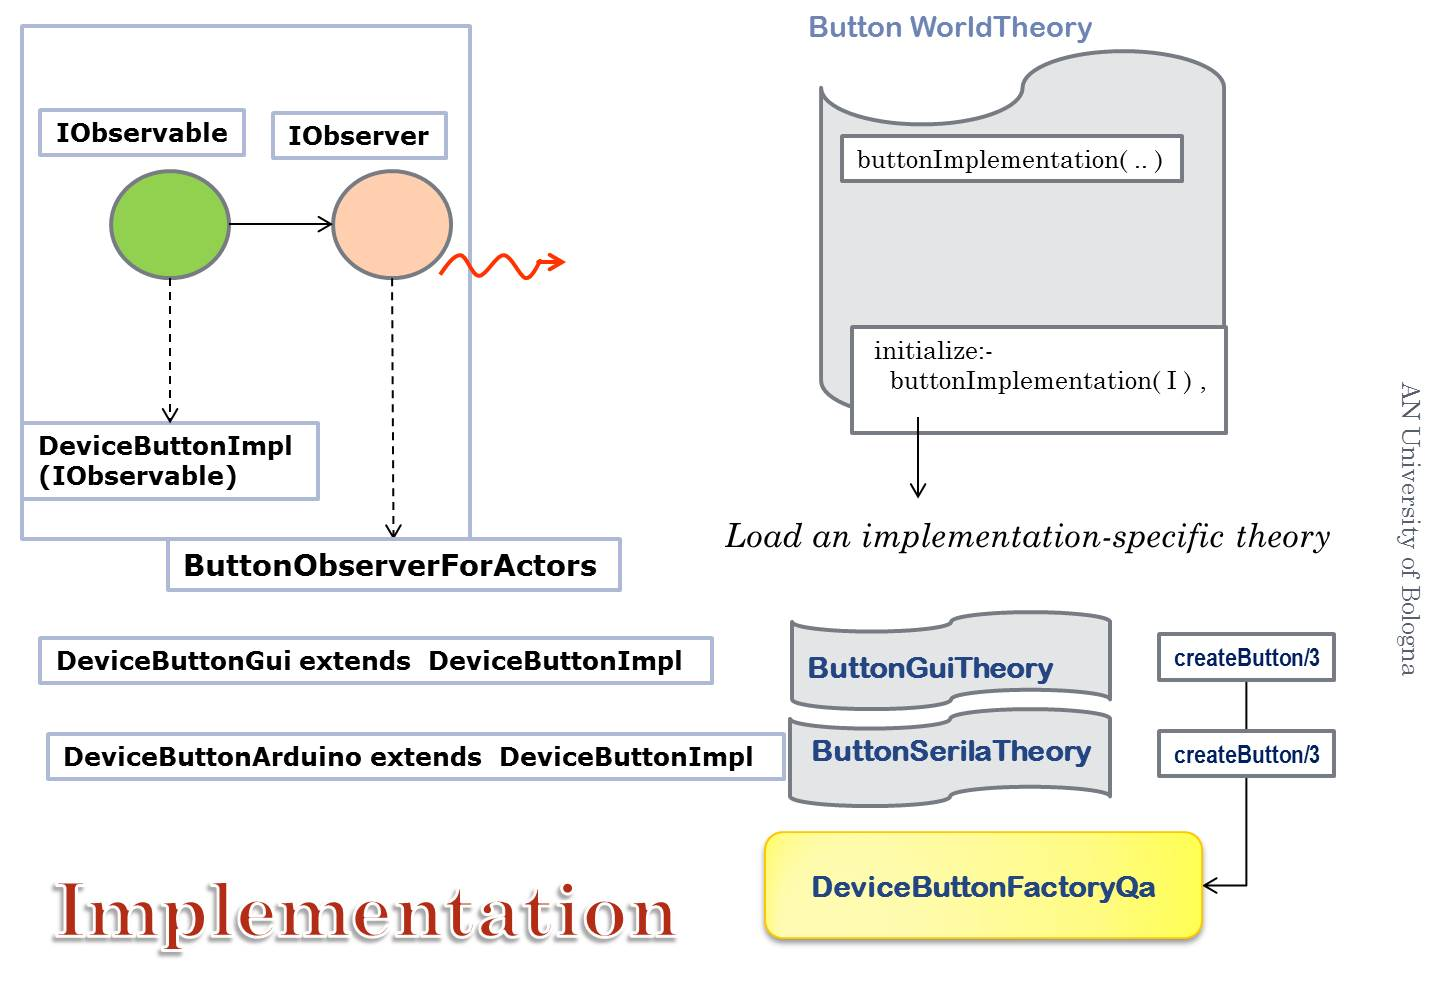
\includegraphics[scale = 0.45]{./img/buttonImplArch.jpg}\\
\end{tabular}{   }
\end{center}

The following picture shows instead the relationship between the implementation layer and the model layer:

\medskip
\begin{center}
\begin{tabular}{ c }
     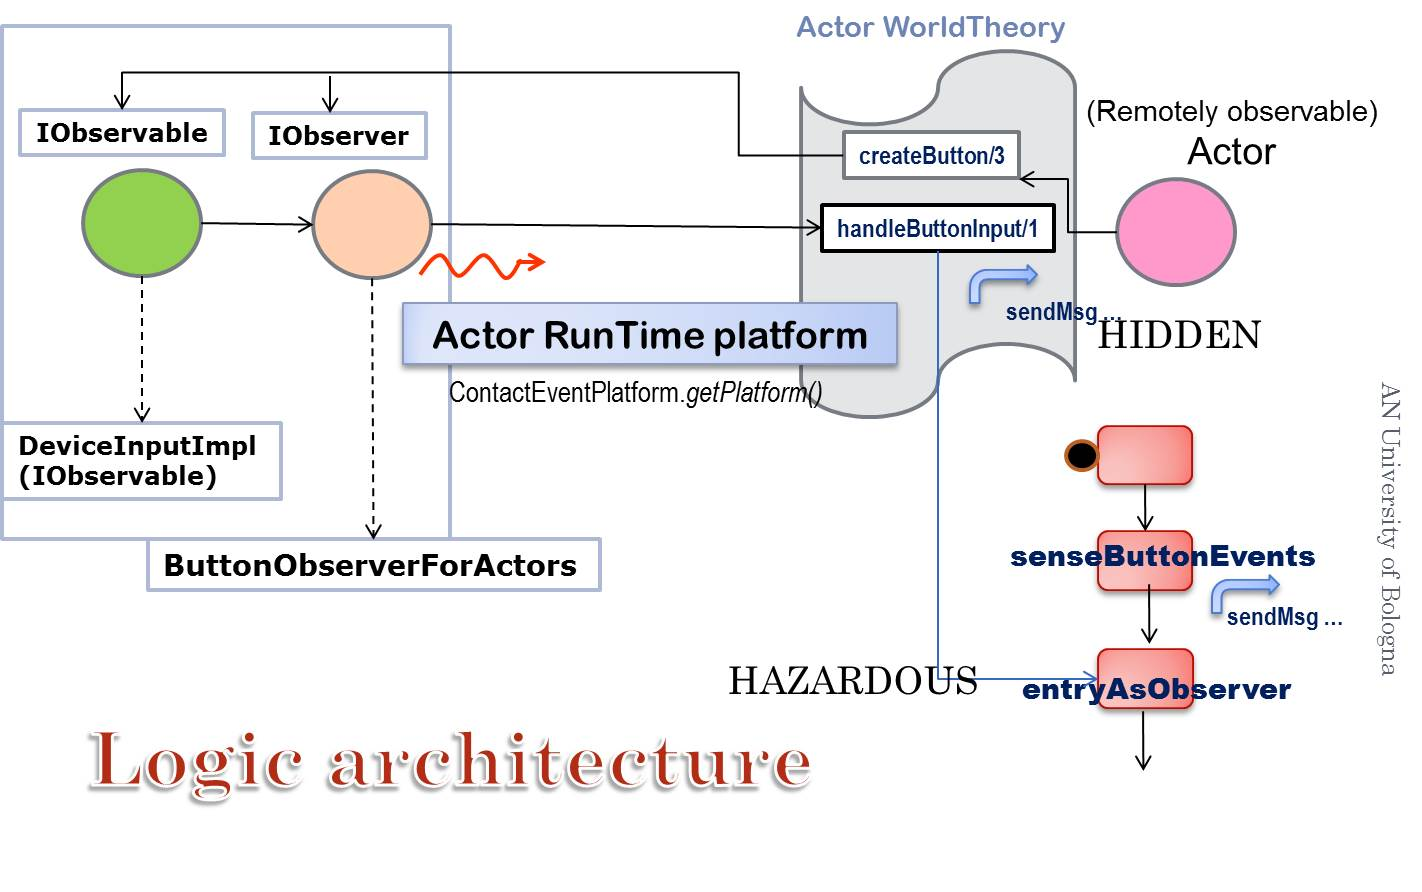
\includegraphics[scale = 0.45]{./img/buttonLogicalArchitecture.jpg}\\
\end{tabular}{   }
\end{center}

\newpage 
\section{A Button factory}
\labelssec{DeviceButtonFactoryQa}
The \java{} class \texttt{DeviceButtonFactoryQa} is a \textit{factory} that provides static methods to create a \textit{singleton} Button object and to get a reference to such an object:

\lstinputlisting[language=java,caption={ \texttt{DeviceButtonFactoryQa.java : createLedMock} }, firstline=1 , lastline=25]{../../../it.unibo.bls2016.device.qa/src/it/unibo/devices/qa/DeviceButtonFactoryQa.java}

Note that any creation method \texttt{createXXX} returns  an object of the class \texttt{DeviceButtonImpl} (see  \xss{DeviceButtonImpl} ). 

\subsection{A basic class for Button implementation}
\labelssec{DeviceButtonImpl}
The \texttt{DeviceButtonImpl} class is based on the custom framework \href{https://137.204.107.21/syskb/it.unibo.iss2015intro/docs/Frameworks/FramwCustomAppl.html}{|>>site/uniboEnv}) introduced for the rapid development of \texttt{GUI}-based prototypes.

\lstinputlisting[language=java,caption={ \texttt{DeviceButtonImpl.java} }, firstline=1 ]{../../../it.unibo.buttonLedSystemHL/src/it/unibo/buttonLed/components/DeviceButtonImpl.java}

\subsection{A Virtual Button (implementation phase)}
A Button as a virtual device can now be introduced as follows:

%%\lstinputlisting[language=java,caption={ \texttt{DeviceButtonGui.java} }, firstline=1 ]{../../../it.unibo.buttonLedSystem.gui/src/it/unibo/buttonLedSystem/gui/DeviceButtonGui.java}

The result is shown in the following picture:

\begin{center}
\begin{tabular}{ c }
     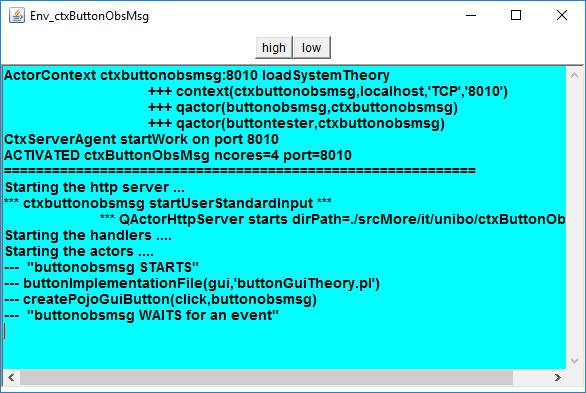
\includegraphics[scale = 0.45]{./img/buttonGui.jpg}\\
\end{tabular}{   }
\end{center}

In order to 'inject' this new implementation of the Button into our logical component, we define the theory \texttt{buttonGuiTheory} with a specific \texttt{createButton/3} rule: 


\lstinputlisting[language=ddr,caption={ \texttt{buttonGuiTheory.pl} }, firstline=1 ]{../../../it.unibo.bls2016.button/buttonGuiTheory.pl}

The next step is to introduce two new rules in  the \texttt{buttonTheory} of \xss{buttonTheory}:

%%\begin{Verbatim}[fontsize=\scriptsize, frame=single , label=Facts related to \texttt{ButtonGui} in \texttt{buttonTheory	}]
\begin{lstlisting}
buttonImplementation( gui ).
...
buttonImplementationFile( gui,  "buttonGuiTheory.pl"   ).
\end{lstlisting}
%%\end{Verbatim}

Finally, we introduce a new button creation operation in the entry in the \texttt{DeviceButtonFactoryQa}:
\lstinputlisting[language=java,caption={ \texttt{DeviceButtonFactoryQa.java : createButtonGui} }, firstline=27 , lastline=36]{../../../it.unibo.bls2016.device.qa/src/it/unibo/devices/qa/DeviceButtonFactoryQa.java}


\newpage 
\section{A Button on Arduino (implementation phase)}

An input device such as the Button can be managed in Arduino in two ways: by polling or via interrupt. 

\subsection{Managing a Button by polling.\\} 

\lstinputlisting[language=java,caption={ \texttt{buttonPolling.ino}}, firstline=1  ]{../../../it.unibo.arduino.intro/Arduino/programs/buttonPolling/buttonPolling.ino} 

\subsection{Managing a Button via interrupt.\\} 

\lstinputlisting[language=java,caption={ \texttt{buttonInterrupt.ino}}, firstline=1  ]{../../../it.unibo.arduino.intro/Arduino/programs/buttonInterrupt/buttonInterrupt.ino} 

\subsection{Managing a Button for qa message-interaction\\} 

\lstinputlisting[language=java,caption={ \texttt{button3Msg.ino}}, firstline=1  ]{../../../it.unibo.arduino.intro/Arduino/programs/button3Msg/button3Msg.ino} 

\subsection{DeviceButtonArduinoProxy}
The class \texttt{DeviceButtonArduinoProxy} creates an object that converts the observed messages coming from an \texttt{Arduino} port  into \texttt{qa} \textit{events} according to the arguments given at creation time:

\lstinputlisting[language=java,caption={ \texttt{DeviceButtonArduinoProxy.java} }, firstline=1 ]{../../../it.unibo.bls2016.device.qa/src/it/unibo/devices/qa/DeviceButtonArduinoProxy.java}

\subsection{Using the serial line in the actor}
In order to 'inject' this new implementation of the Button into our logical component, we define the theory \texttt{buttonSerialTheory} with a specific \texttt{createButton/3} rule: 


\lstinputlisting[language=ddr,caption={ \texttt{buttonGuiTheory.pl} }, firstline=1 ]{../../../it.unibo.bls2016.button/buttonSerialTheory.pl}

The next step is to introduce two new rules in  the \texttt{buttonTheory} of \xss{buttonTheory}:

%%\begin{Verbatim}[fontsize=\scriptsize, frame=single , label=Facts related to \texttt{ButtonGui} in \texttt{buttonTheory	}]
\begin{lstlisting}
buttonImplementation( arduino ).
...
buttonImplementationFile( arduino,  "buttonSerialTheory.pl"   ).
\end{lstlisting}
%%\end{Verbatim}

Finally, we introduce a new button creation operation in the entry in the \texttt{DeviceButtonFactoryQa}:
\lstinputlisting[language=java,caption={ \texttt{DeviceButtonFactoryQa.java : createButtonSerialProxy} }, firstline=47 , lastline=54]{../../../it.unibo.bls2016.device.qa/src/it/unibo/devices/qa/DeviceButtonFactoryQa.java}


 

\newpage 
\section{A Button on Raspberry (implementation phase)}
In this example, one terminal of the Button is connected to the \texttt{5V} pin (physical pin 2) while the other one (button-input pin) to pin \texttt{24} in \texttt{BCM} code. A resistor  of \texttt{10K} ohm\footnote{10K colors: brown, black, orange and argent/gold} )  is also inserted between the input pin and a \texttt{GND} pin (e.g. physical pin 9) to assure a connection to the ground when the button is not pressed.

\subsection{Button control using files}
The basic way provided by Linux to manage a device connected on a \texttt{GPIO} pin is reading/writing some (virtual) file associated with that pin.

\lstinputlisting[language=ddr,caption={ \texttt{buttonOn24Click.sh} }, firstline=1 ]{../../../it.unibo.raspIntro/src/it/unibo/bls/bash/buttonOn24Click.sh}



\subsection{Button control using the \texttt{GPIO} shell library}
The \texttt{gpio} library allows us to write a program (bash file) that reads the button-input pin and writes a \texttt{0/1} value on the Led pin:

\lstinputlisting[language=ddr,caption={ \texttt{button24Gpio.sh} }, firstline=1 ]{../../../it.unibo.raspIntro/src/it/unibo/bls/bash/gpio/button24Gpio.sh}

\subsection{Button control using python}
The Python library that handles interfacing with the \texttt{GPIO} pins allows us to write:

\lstinputlisting[language=ddr,caption={ \texttt{buttonPython24.py} }, firstline=1 ]{../../../it.unibo.raspIntro/src/it/unibo/bls/python/buttonPython24.py}



\subsection{Button control using Pi4j}
The \texttt{Pi4J} library (see \href{https://137.204.107.21/syskb/it.unibo.iss2015intro/docs/Raspberry/pi4j.html}{|>>site/Pi4j}) can be used as our \textit{technology assumption} for the implementation a \java{} class for the control of a Button connected to some pin of a Raspberry Pi:

\lstinputlisting[language=java,caption={ \texttt{DeviceLedPi4j.java} }, firstline=1 , lastline=55]{../../../it.unibo.buttonLedSystem.raspberry/src/it/unibo/bls/raspberry/components/DeviceButtonPi4j.java}

\subsection{Using the Button Pi4j in the actor}
In order to 'inject' this new implementation of the Led into our logical component, we define the theory \texttt{buttonPi4jTheory.pl}:

\lstinputlisting[language=ddr,caption={ \texttt{ledPi4jTheory.pl} }, firstline=1 ]{../../../it.unibo.bls2016.button/buttonPi4jTheory.pl}

The next step is to introduce two new rules in  the \texttt{ledTheory} of \xss{ledTheory}:

%%\begin{Verbatim}[fontsize=\scriptsize, frame=single , label=Facts related to \texttt{LedMock} in \texttt{ledTheory	}]
\begin{lstlisting}
buttonImplementation( rasp ).
...
buttonImplementationFile( rasp, "buttonPi4jTheory.pl"  ).
\end{lstlisting}
%%\end{Verbatim}

 

Finally, we introduce a new button creation operation in the entry in the \texttt{DeviceButtonFactoryQa}:
\lstinputlisting[language=java,caption={ \texttt{DeviceButtonFactoryQa.java : createButtonPi4j} }, firstline=38 , lastline=45]{../../../it.unibo.bls2016.device.qa/src/it/unibo/devices/qa/DeviceButtonFactoryQa.java}

\newpage 
\section{A Button as an observable}
\labelsec{btnobservable}
 
In our first actor-based model (see \xss{buttonasactor}) the button sends a message to a single (remote) actor. In that case, our effort was focussed on the relationship between the button-actor and the embedded button-\texttt{POJO}. In particular, the button-\texttt{POJO} has been conceived as an observable (\texttt{GOF}) object, and the \texttt{ButtonObserverForActors} defined in \xss{bobsqa} has been introduced to perform (when the button changes its state) two basic actions:
\begin{enumerate}
\item emit an event \texttt{eventId:eventMsg} (values given at creation time)  ;
\item solve the goal \texttt{handleButtonInput/1} in order to delegate to the button-actor the handling of the current button state.
\end{enumerate}

Therefore, our button-actor \texttt{buttonobsmsg} is already able to interact with any other local or remote actor that decides to sense the \texttt{eventId:eventMsg}.  In other words, the button-actor is already 'observable' by other actors, thanks to the underlying \texttt{qa} event support.

In the following model we want modify the behaviour of our button so that is becomes also able to interact with \texttt{P2P} messages with other actors that explicitly manifest (via a 'registration') their intention to receive updating massages.

\lstinputlisting[language=ddr,caption={ \texttt{buttonObservable.qa} }, firstline=1, lastline=43]{../../../it.unibo.bls2016.button/src/buttonObservable.qa}

The \texttt{buttonobservable} does not need to know its observers. The observers can be dynamically added to a system(see \xs{dynsys}) that initially starts with the Button as unique component. When the Button registers an observer,  the knowledge-base about the current system configuration is shown by the operation \texttt{showSystemConfiguration} introduced in \xss{sysconfshow}.

When the (embedded \texttt{POJO}) button changes its state, the \texttt{entryAsObserver} Plan is called and the Button sends an asynchronous  message to each registered observer as specified in the   \texttt{updateOps} rule of the \texttt{observableTheory}:

\lstinputlisting[language=pl,caption={ \texttt{observableTheory.pl} }, firstline=1,lastline=25]{../../../it.unibo.bls2016.button/observableTheory.pl}

 
To test the \texttt{buttonObservable} we can introduce some local observer actor:

\lstinputlisting[language=ddr,caption={ \texttt{buttonObservable.qa: an observer} }, firstline=45, lastline=55]{../../../it.unibo.bls2016.button/src/buttonObservable.qa}


\subsection{A Led as an observer}

Now that we have extended the \texttt{GOF} observer pattern to a distributed environment, we can dynamically introduce (see \xs{dynsys}) a remote Led that works as a button observer, by looking either at  messages or at  events.

\lstinputlisting[language=ddr,caption={ \texttt{ledAsObserver.qa} }, firstline=1 ]{../../../it.unibo.bls2016.button.observer/src/ledAsObserver.qa}

\newpage 
\section{Towards dynamic systems}
\labelsec{dynsys}
The flag \texttt{-standalone} in the declaration of a Context indicates that all the actors defined in that context must be considered external to the current system and (perhaps) already in existence. Thus, the  actors defined in a \texttt{-standalone} Context are 'place holders' for reference purposes (e.g. message passing, that requires a reference to an actor name).

The ButtonLed introduced in \xs{btnobservable} is an example of a dynamic system that can be incrementally expanded. The first logical step consists in activating the Button as a (standalone) observable entity. In the next step, a number of Leds  can be activated, each working (in its own computational) node as an observer that must 'register' itself to the Button. 


\subsection{Updating the system knowledge base}
\labelssec{sysconfkb}

Each time that a new component is dynamically added to the system, the system knowledge-base stored in each Context\footnote{The static part of the system knowledge is stored in a file \texttt{projectname,pl} generated  in the Context package of the directory \texttt{srcMore}.} is dynamically extended by the \texttt{qa} run-time support with the configuration 	related to the new component.
%
In this way, each actor in the system becomes able to send messages to other remote actors (dynamically introduced in the system), if it is able to know their names\footnote{The \texttt{register} message sent by a Led to the Button is the way used to make the Button aware of the name of the Led.} 

With reference to the ButtonLed, the initial knowledge-base related to the observable Button\footnote{The initial knowledge-base of the Button is generated in the file \textit{srcMore/it/unibo/ctxButtonObservable/buttonobservable.pl}}  is: 

\lstinputlisting[language=pl,caption={ \texttt{buttonobservable.pl of ctxButtonObservable} }, firstline=1,lastline=24]{../../../it.unibo.bls2016.button/srcMore/it/unibo/ctxButtonObservable/buttonobservable.pl}


The initial knowledge-base related to a Led\footnote{The initial knowledge-base of the observer Led is generated in the file \textit{srcMore/it/unibo/ctxLedAsObserver/ledasobserver.pl}} is:

\lstinputlisting[language=pl,caption={ \texttt{ledasobserver.pl of ctxLedAsObserver } }, firstline=1]{../../../it.unibo.bls2016.button.observer/srcMore/it/unibo/ctxLedAsObserver/ledasobserver.pl}


\subsection{Getting the system-configuration at application level}
\labelssec{sysconfshow}

The knowledge about a context configuration can be acquired at application level by rules like the following ones:

\lstinputlisting[language=pl,caption={ \texttt{observableTheory.pl} }, firstline=26]{../../../it.unibo.bls2016.button/observableTheory.pl}
 
When the Led is added to the system,  the knowledge-base of the Button is shown as follows\footnote{The actors whose names stars with \texttt{evlpa} are internal actors of class \texttt{EventLoopActors} that implement event-handling including system events.} :

\begin{lstlisting}
--- CURRENT CONTEXTS:
--- context(ctxbuttonobservable,localhost,'TCP','8010')
--- context(ctxledasobserver,localhost,'TCP','8043')
--- CURRENT ACTORS:
--- qactor(buttonobservable,ctxbuttonobservable)
--- qactor(btnobserver1,ctxbuttonobservable)
--- qactor(evlpactxbuttonobservable,ctxbuttonobservable)
--- qactor(ledobserver,ctxledasobserver)
--- qactor(evlpactxledasobserver,ctxledasobserver)
\end{lstlisting}

The same knowledge-base is updated in the Led site (and all in the other nodes dynamically added to the system).

\newpage 
\section{A system based on events}
The button-\texttt{POJO} embedded in the Button actor is an observable (\texttt{GOF}) object associated with a 'listener' (\texttt{ButtonObserverForActors}, see \xss{bobsqa}) that emits an event \texttt{eventId:eventMsg} (values given at creation time).
%
Therefore, our button-actor is already an 'observable' entity and any other local or remote actor that decides to sense the \texttt{eventId:eventMsg} can be work as a button observer.   

Thus, the logical architecture of the ButtonLed system can be redefined as follows.

\subsection{The Button as an event emitter}
The Button can be defined as an actor that emits the event \texttt{clicked:clicked(click)}. A first prototype (useful in our first sprint review) can be introduces by selecting the \texttt{GUI} implementation of the Button:   

\lstinputlisting[language=ddr,caption={ The Button as an event emitter \texttt{buttonEvent.qa} }, firstline=1 ]{../../../it.unibo.bls2016.button/src/buttonEvent.qa}

The Button Plan (state) \texttt{senseButtonEvents} does not perform here any interesting action and could be completely omitted. However, a more significant Button behaviour is introduced in \xs{usemqtt}.

Since the Button can be observed by any new component that decides to perceive the \texttt{clicked} event we can immediately starts to run the button without any observer:

\begin{tabular}{|c|c|}
\hline 
The Button & The Led \\ 
\hline 
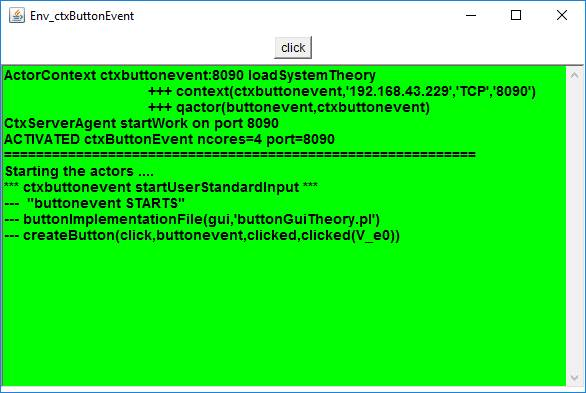
\includegraphics[scale = 0.4]{./img/buttonEventGui.jpg}
  &  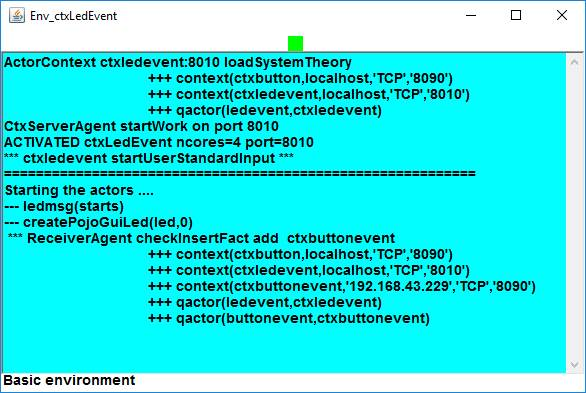
\includegraphics[scale = 0.40]{./img/ledEventGui.jpg} \\
\hline 
\end{tabular} 
\subsection{The Led as an event perceiver}
The Led can be defined as actor that waits for a clicked event and then, when the event is perceived, switches its state. Also in this case our first prototype is based on the \texttt{GUI} implementation of the Led:

\lstinputlisting[language=ddr,caption={ \texttt{ledEvent.qa} }, firstline=1 ]{../../../it.unibo.bls2016.led/src/ledEvent.qa}

Note that the button context is declared as \texttt{-standalone}. In this case we do not introduce any place holder (for the Button) since we don't have any direct interaction with it.
 
\newpage 
\section{A Button on Android}
\labelsec{buttonandroid} 
The \texttt{ButtonObserverForActors} of \xss{bobsqa} is a 'listener' that we can add also to a Button-\texttt{POJO} implemented on an Android system. According to our work-plan, we can introduce the following (in \texttt{SCRUM} terminology) \textit{product-backlog}:

\begin{itemize}
\item update the \texttt{buttonTheory} of \xss{buttonTheory} by introducing new facts related to the implementation of a Button-\texttt{POJO} in a Android environment:

%%\begin{Verbatim}[fontsize=\scriptsize, frame=single , label=Facts related to \texttt{ButtonGui} in \texttt{buttonTheory	}]
\begin{lstlisting}
buttonImplementation( android ).
...
buttonImplementationFile( gui,  "buttonAndroidTheory.pl"   ).
\end{lstlisting}
%%\end{Verbatim}

\item define the \texttt{buttonAndroidTheory}:
\lstinputlisting[language=ddr,caption={ \texttt{buttonAndroidTheory.pl} }, firstline=1 ]{../../../it.unibo.android.button.qa/assets/it/unibo/buttonqaandroid/buttonAndroidTheory.pl}

The rule \texttt{createButton/3} does not use any more the \texttt{class("...") <- op(...)} mechanism\footnote{ The \texttt{tuProlog} requires some modification of usage (see tuProlog manual, section \texttt{3.4}) in an Android environment} , but explicitly delegates the creation of the button to an operation (\texttt{createButton})  to be defined by the application designer within the actor so to adapt this task to the rules of the Android environment.

\item define an implementation for the button for Android as a specialization of the class \texttt{DeviceButtonImpl} of \xss{DeviceButtonImpl}.

\end{itemize}

\subsection{The implementation}

For the sake of simplicity, we do not use  any more the \texttt{DeviceButtonFactoryQa} of \xss{DeviceButtonFactoryQa}. Rather, we do introduce a factory method (\texttt{createButtonAndroid}) in the class \textit{DeviceButtonAndroid}. 

\lstinputlisting[language=java,caption={ \texttt{DeviceButtonAndroid.java} }, firstline=1 ]{../../../it.unibo.android.button.qa/src/it/unibo/android/button/DeviceButtonAndroid.java}

This factory method is called by the \texttt{createButton} operation that should be defined by the Application designer in the generated button implementation class \texttt{Buttonqaandroid}:

\lstinputlisting[language=java,caption={ \texttt{Buttonqaandroid.java} }, firstline=1 ]{../../../it.unibo.android.button.qa/src/it/unibo/buttonqaandroid/Buttonqaandroid.java}

The class \texttt{Buttonqaandroid} is generated only once, as a specialized version of an abstract class that implements the behaviour defined in the model.

\subsection{A model}
\labelssec{androqamodel}
Let us introduce here model similar to that of \xs{btnobservable}:

\lstinputlisting[language=ddr,caption={ \texttt{buttonAndroid.qa} }, firstline=1 ]{../../../it.unibo.android.button.qa/src/buttonAndroid.qa}

\bigskip 
\subsection{The software factory under Android}

Let us start by creating a new Android Application Project\footnote{We suppose to work in \textit{Eclipse/Xtext} extended with the \texttt{qa} plugins.}. 

\medskip   
\begin{tabular}{|c|c|}
\hline 
Android Application project 1 & Android Application project 2 \\ 
\hline 
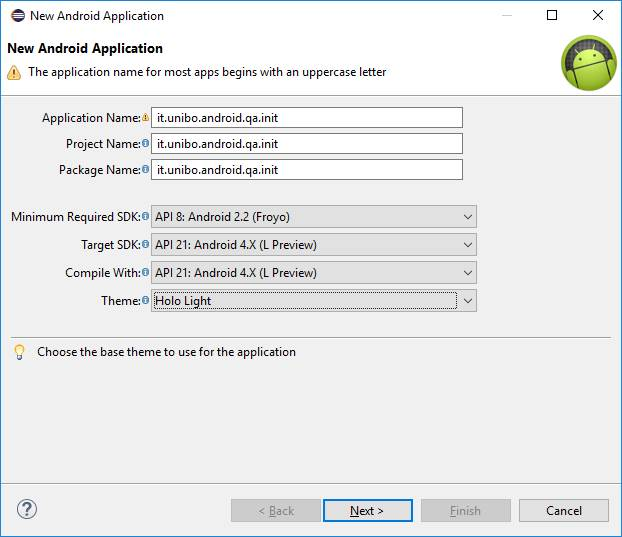
\includegraphics[scale = 0.45]{./img/qainitAndroid0.jpg}
  &  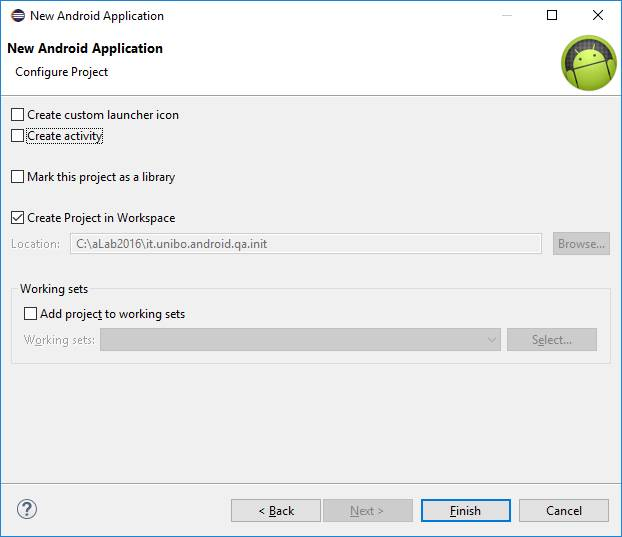
\includegraphics[scale = 0.45]{./img/qainitAndroid1.jpg} \\
\hline 
\end{tabular} 
\medskip 

If we introduce a \texttt{qa} model, a set of resources is generated, including a file \textit{AndroidManifestCustom.xml} whose content must replace the content of the \textit{AndroidManifest.xml} generated by the \texttt{AIDE} (Android \texttt{IDE}):

\medskip 
\begin{tabular}{|c|c|}
\hline 
Define a \texttt{qa} model & Code generated \\ 
\hline 
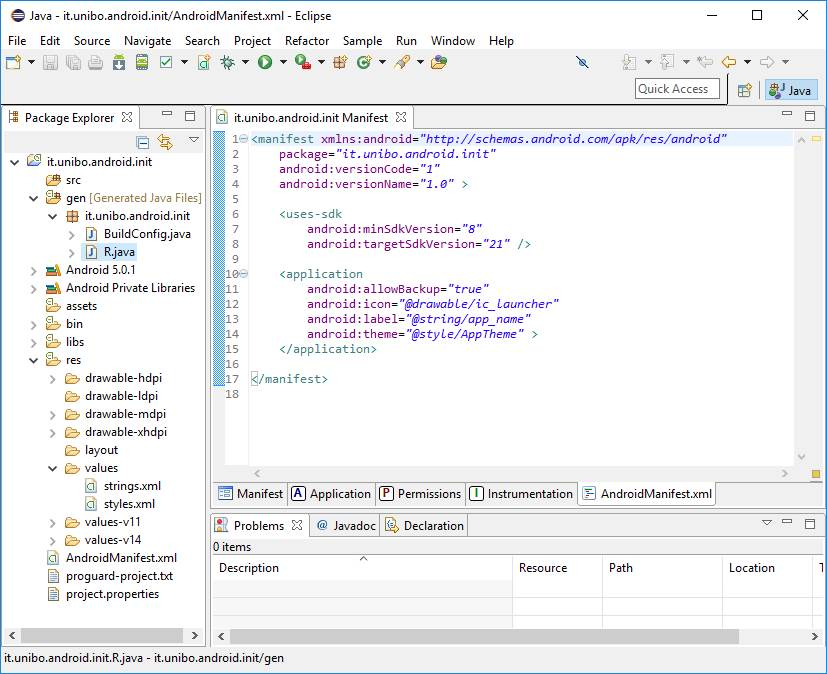
\includegraphics[scale = 0.35]{./img/qainitAndroid2.jpg}
  &  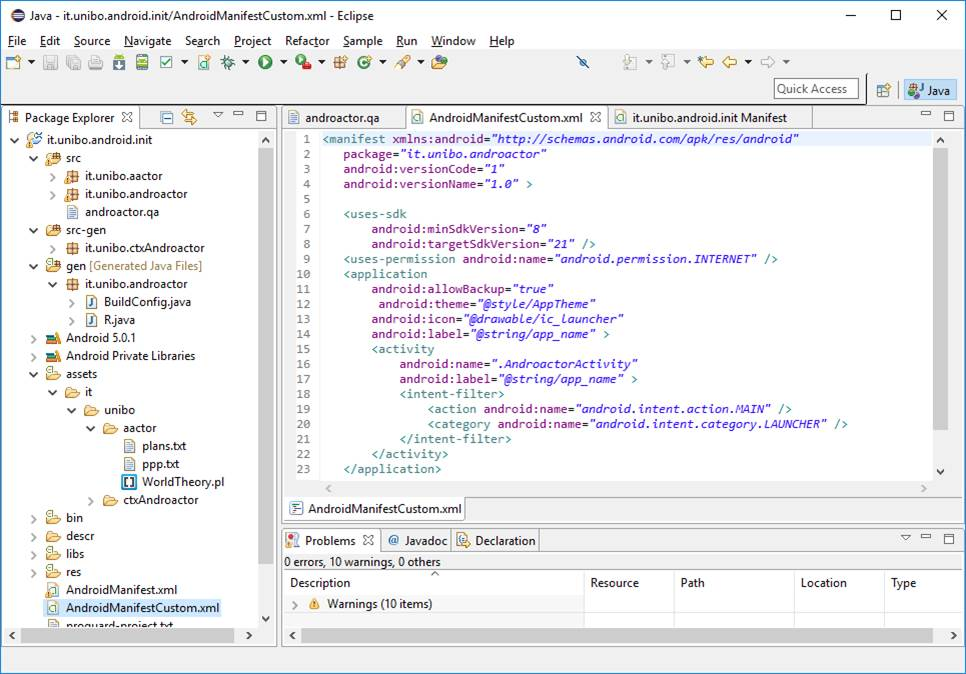
\includegraphics[scale = 0.30]{./img/qainitAndroid3.jpg} \\
\hline 
\end{tabular}
\medskip 

Note that the \texttt{srcMore} directory now does not exist any more; its content is now generated in the \texttt{assets} Android directory.
Moreover, a \texttt{xml} file (whose name \textbf{\textit{must}} be written in lower-case letters) is now generated in the Android directory \texttt{res/layout} to include the specification of a 'standard' \texttt{GUI} for the \texttt{qa} application, that forces an updating (by the  \texttt{AIDE})of the \texttt{R.java} file in the \texttt{gen} directory.
  
In the  \texttt{src} directory we can find an Activity (that extends the generated \texttt{BaseActivity} class), that defines the skeleton of the main application activity. This activity is generated only once; the task of the Application designer is to complete this code according to application needs.

Here is the structure of the project workspace for the model of \xss{androqamodel}.

\textbf{Project workspace.}\\
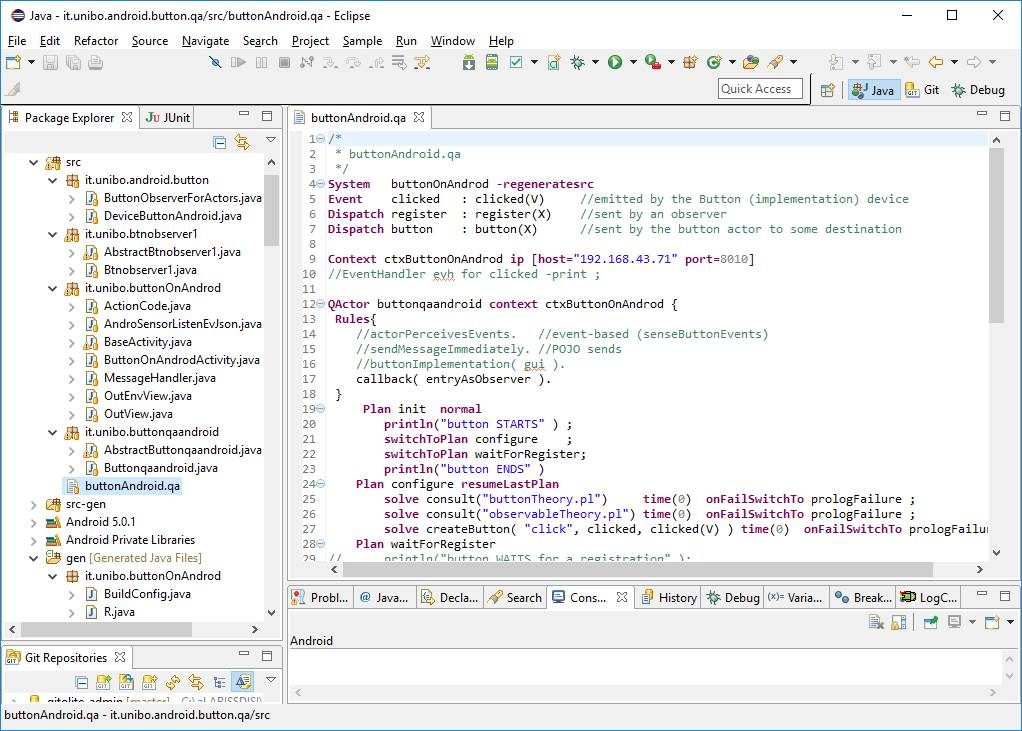
\includegraphics[scale = 0.40]{./img/qainitAndroid4.jpg}
 

\textbf{Libraries involved.} \\
 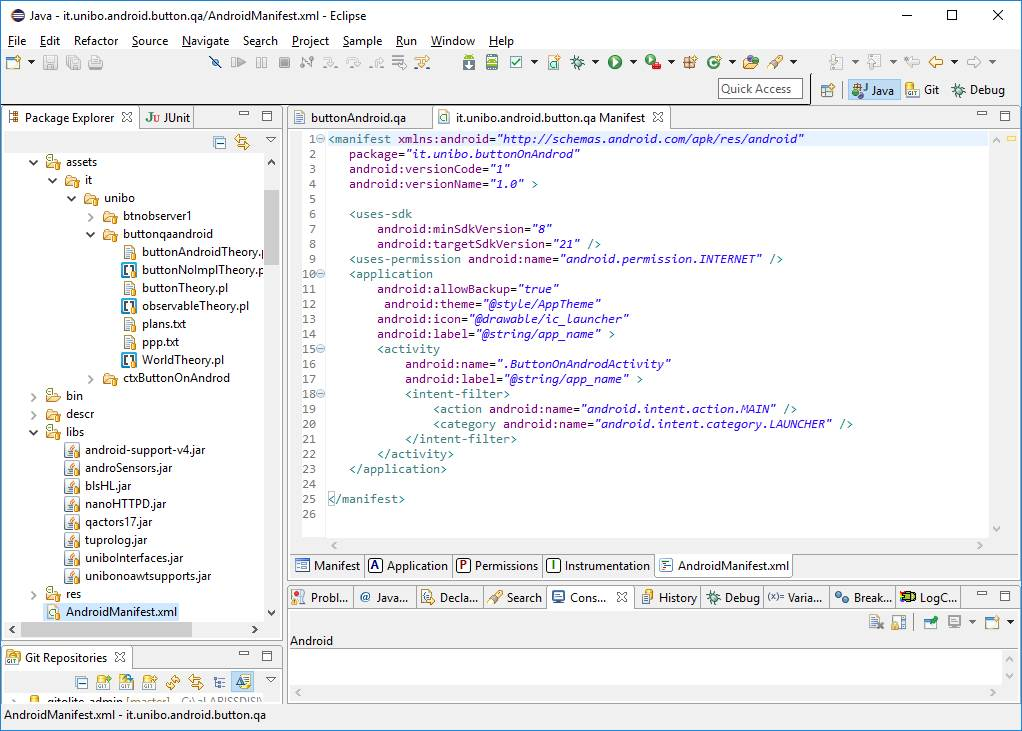
\includegraphics[scale = 0.40]{./img/qainitAndroid5.jpg}
 

\newpage 
\section{Interactions using \texttt{MQTT}}
\labelsec{usemqtt}
In this section we will redesign the remotely-observable Button of \xs{btnobservable} as an actor that works also as a \textit{publisher} of information  by using the \texttt{MQTT} protocol.

The \texttt{MQ} \textit{Telemetry Transport} (\texttt{MQTT}) is an ISO standard (ISO/IEC PRF 20922) publish-subscribe based "light weight" messaging protocol for use on top of the TCP/IP protocol. It is useful for connections with remote locations where a small code footprint is required and/or network bandwidth is at a premium.

The \textit{Eclipse Paho} project provides open-source client implementations of \texttt{MQTT} and \texttt{MQTT-SN} (\textit{MQTT For Sensor Networks}\footnote{\texttt{MQTT-SN} is a protocol derived from \texttt{MQTT}, designed for connectionless underlying network transports such as \texttt{UDP}}) messaging protocols aimed at new, existing, and emerging applications for \textit{Machine-to-Machine} (\texttt{M2M}) and \textit{Internet of Things} (\texttt{IoT}). There are already \texttt{MQTT} \texttt{C} and \java{} libraries with \texttt{Lua}, \texttt{Python}, \texttt{C++} and \texttt{JavaScript} at various stages of development.

\subsection{The Button as a \texttt{MQTT} publisher}
The remotely-observable Button introduced in \xs{btnobservable} is here extended (see the Plan \texttt{configure} and the Plan \texttt{entryAsObserver}) to become (when it changes its state) a \texttt{MQTT} publisher of information on the topic \texttt{"unibo/button/qa"}.

\lstinputlisting[language=ddr,caption={ The Button as a \texttt{MQTT} publisher \texttt{buttonMqtt.qa} }, firstline=1 ]{../../../it.unibo.bls2016.button.mqtt/src/buttonMqtt.qa}

The usage of the \texttt{MQTT} protocol is delegated to rules defined by the application designer in the \texttt{mqttTheory}. These rules in their turn make use of a \java{} utility object of class \texttt{MqttUtils}.

\subsection{The MqttUtils}
The \java{} utility class to be used as a support for \texttt{MQTT} interaction can be defined as follows:

\lstinputlisting[language=java,caption={ The utility class \texttt{MqttUtils.java} }, firstline=1 ]{../../../it.unibo.bls2016.button.mqtt/src/it/unibo/mqtt/utils/MqttUtils.java}

An object of class \texttt{MqttUtils} is used as a \textit{singleton} and works as the support for the actor that calls the operation \texttt{connect} (that creates a \texttt{MqttClient}).

The \texttt{subscribe} operation sets this singleton support as the object that provides the callback (\texttt{messageArrived}) to be called when the \texttt{MqttClient} is a subscriber. The callback is defined so to map a \texttt{MqttMessage} into a dispatch of the form:

\begin{Verbatim}[fontsize=\scriptsize, frame=single]
mqttmsg : mqttmsg( TOPIC,PAYLOAD )
\end{Verbatim}

This dispatch is then sent to the actor that uses the singleton support, i.e. that works as a \texttt{MqttClient} (subscriber).

\subsection{The mqttTheory}
The \texttt{mqttTheory} that 'extends' the \texttt{qa} action-set with new operations for the usage of the \texttt{MQTT} protocol can be defined as follows:

\lstinputlisting[language=pl,caption={ The \texttt{mqttTheory.pl} }, firstline=1 ]{../../../it.unibo.bls2016.button.mqtt/mqttTheory.pl}



\subsection{A Button observer as a \texttt{MQTT} subscriber}
To test the behaviour of our new Button-publisher, let us introduce an observer as a \texttt{MQTT} subscriber:

\lstinputlisting[language=ddr,caption={ \texttt{observerMqtt.qa} }, firstline=1 ]{../../../it.unibo.bls2016.button.mqtt/src/observerMqtt.qa}

\subsection{A Button observable actor} 
\labelssec{btnmodelandroid}
Of course we can introduce also a conventional actor that works as a Button observer via the 'registration' mechanism of \xs{btnobservable}:

\lstinputlisting[language=ddr,caption={ \texttt{observerQa.qa} }, firstline=1 ]{../../../it.unibo.bls2016.button.observer/src/observerQa.qa}




\newpage 
\section{From the components to the systems}
\labelsec{tosystem}




 